% =====================================================================
% Segunda parte – 4. Pruebas de integración
% =====================================================================
\section{Pruebas de integración}

\subsection{Estrategia incremental ascendente}

Integramos de abajo hacia arriba siguiendo las capas del backend (Figura \ref{fig:integracion}). Cada nivel se prueba con los inferiores ya verificados y con un \emph{driver} que reemplaza al nivel superior; no se necesitan \emph{stubs} porque se parte de la capa sin dependencias.

\begin{figure}[H]
\centering
\caption{Esquema de integración incremental ascendente de ShiftCash}
\label{fig:integracion}
\resizebox{\linewidth}{!}{%
\begin{tikzpicture}[
  nivel/.style={caja, text width=4.6cm, minimum height=1.1cm},
  drv/.style={caja, cajagris, text width=4.4cm, minimum height=1.1cm, font=\scriptsize},
]
\node[nivel] (l1) at (0,0) {\textbf{N1.} \codigo{models.py} + \codigo{database.py}\\(SQLite con FK activadas)};
\node[nivel] (l2) at (0,1.8) {\textbf{N2.} + \codigo{schemas.py}\\(validación Pydantic)};
\node[nivel, cajaacento] (l3) at (0,3.6) {\textbf{N3.} + \codigo{services/}\\(presupuestos, metas, categorías)};
\node[nivel] (l4) at (0,5.4) {\textbf{N4.} + \codigo{auth.py} + \codigo{routes/}\\(API REST con JWT)};
\node[nivel] (l5) at (0,7.2) {\textbf{N5.} + cliente \codigo{api/*.js}\\(Axios + JWT)};
\node[nivel] (l6) at (0,9) {\textbf{N6.} + hooks, vistas y modales\\(SPA completa)};
\foreach \a/\b in {l1/l2, l2/l3, l3/l4, l4/l5, l5/l6} \draw[flecha] (\a) -- (\b);
\node[drv] (d1) at (6.6,1.8) {Driver: \codigo{test_unitarias.py} (esquemas y funciones puras)};
\node[drv] (d2) at (6.6,4.5) {Driver: \codigo{TestClient} de FastAPI en \codigo{test_integracion.py} (39 pruebas)};
\node[drv] (d3) at (6.6,7.2) {Driver: \codigo{cy.request} de Cypress contra la API en ejecución};
\node[drv] (d4) at (6.6,9) {Driver: navegador de Cypress y Selenium};
\draw[flechapunteada] (d1) -- (l2); \draw[flechapunteada] (d2) -- (l3.east); \draw[flechapunteada] (d2) -- (l4.east);
\draw[flechapunteada] (d3) -- (l5); \draw[flechapunteada] (d4) -- (l6);
\node[font=\scriptsize\itshape, rotate=90] at (-3.2,4.5) {orden de integración};
\draw[-{Stealth[length=3mm]}, gris, very thick] (-2.8,0) -- (-2.8,9);
\end{tikzpicture}}
\figurenote{Fuente: elaboración propia.}
\end{figure}

\subsection{Estrategia basada en hilos}

\begin{table}[H]
\caption{Hilos de integración}
\label{tab:hilos}
\footnotesize
\begin{tabularx}{\linewidth}{L{1cm} L{2.2cm} Y}
\toprule
Hilo & Caso de uso & Recorrido \\
\midrule
H1 & CU01, CU08 & ModalTransaccion → \codigo{useTransaccionForm} → \codigo{POST /transactions/} → \codigo{category_service} → BD → historial y resumen \\
H2 & CU01 + CU02 & Gasto → \codigo{GET /budgets/} → \codigo{budget_service.calculate_spent} → tarjeta con porcentaje real \\
H3 & CU03, CU13 & MetaFormModal → \codigo{POST /saving-goals/} → \codigo{generate_daily_amounts} → plantilla del reto → \codigo{toggle-day} → progreso \\
H4 & CU14 & Transacción recurrente → \codigo{registrar_recurrentes} → instancia del día \\
H5 & CU04–CU07, CU12 & Registro, inicio de sesión (con Google simulado), perfil, categorías y eliminación en cascada \\
\bottomrule
\end{tabularx}
\tablenote{Fuente: elaboración propia.}
\end{table}

\subsubsection{Análisis del hilo H3: tabla de estados y tabla de valores}

El hilo H3 recorre CU03 y CU13 (crear una meta y marcar los días del reto); su diagrama de secuencia es la Figura \ref{fig:sec-cu03}. Una meta no tiene un campo de estado: su estado se deduce de los días marcados ($d$) frente a los días del plan ($N$).

\begin{table}[H]
\caption{Tabla de estados de una meta de ahorro (hilo H3)}
\label{tab:estados-h3}
\footnotesize
\begin{tabularx}{\linewidth}{L{2.4cm} L{3.4cm} L{2.6cm} Y}
\toprule
Estado actual & Evento & Estado siguiente & Respuesta del sistema \\
\midrule
E0 Sin meta & Crear meta válida & E1 Creada ($d = 0$) & 200; plan de $N$ cuotas que suman el objetivo \\
E0 Sin meta & Crear meta con monto no redondo o fechas invertidas & E0 & 422 con el motivo (PA-08) \\
E1 Creada & Marcar un día $k$ con $1 \leq k \leq N$ & E2 En progreso & 200; sube el ahorro en la cuota del día $k$ \\
E2 En progreso & Marcar otro día válido & E2, o E3 si $d = N$ & 200; E3 cuando el ahorro llega al 100\,\% \\
E2 En progreso & Desmarcar el único día marcado & E1 & 200; el ahorro vuelve a 0 \\
E3 Completada & Desmarcar un día & E2 & 200; el ahorro baja \\
E1, E2 o E3 & Marcar un día que no existe ($k < 1$ o $k > N$) & El mismo & 422 «Ese día no pertenece al plan» (D-15) \\
E1, E2 o E3 & Editar el objetivo o la fecha final & E1 o E2 & 200; se rehace el plan y los días fuera del plan nuevo dejan de contar (D-15) \\
E1, E2 o E3 & Eliminar la meta & E0 & 200 \\
\bottomrule
\end{tabularx}
\tablenote{Fuente: elaboración propia a partir de \codigo{services/saving_service.py}.}
\end{table}

La tabla de valores aplica valores límite al número de día y a los datos de la meta, con una meta de \$5\,000 y 5 días ($N = 5$).

\begin{table}[H]
\caption{Tabla de valores del hilo H3}
\label{tab:valores-h3}
\footnotesize
\begin{tabularx}{\linewidth}{L{2.2cm} L{1.6cm} L{3.4cm} L{3cm} Y}
\toprule
Entrada & Valor & Resultado esperado & Obtenido antes (26/11/2026) & Obtenido después \\
\midrule
Día & 1 (límite inferior) & 200; $d = 1$ & 200; $d = 1$ & 200; $d = 1$ \\
Día & 5 (límite superior) & 200; $d$ aumenta en 1 & 200 & 200 \\
Día & 3 dos veces & Marca y luego desmarca & Marca y desmarca & Marca y desmarca \\
Día & 0 & 422 & \textbf{200; $d$ aumenta sin ahorro} & 422 \\
Día & $-1$ & 422 & \textbf{200; $d$ aumenta} & 422 \\
Día & 6 ($N + 1$) & 422 & \textbf{200; $d$ aumenta} & 422 \\
Día & 99 & 422 & \textbf{200; queda $d = 3$ de 5 sin ningún día válido} & 422 \\
Fecha final & Acortada a 2 días con el día 5 marcado & El día 5 deja de contar & \textbf{Seguía contando} & \codigo{completed_days} vacío \\
Objetivo & 1\,500 & 422 (múltiplo de 1\,000) & 422 & 422 \\
Fecha final & Vacía & Plan de 30 días (D-07) & 30 días & 30 días \\
\bottomrule
\end{tabularx}
\tablenote{En negrita, los resultados que no coinciden con lo esperado: son el defecto D-15, corregido en \codigo{toggle_day} y \codigo{update_goal} con la prueba de regresión \codigo{test_d15_marcar_dia_fuera_del_plan_422}, que fallaba antes del cambio. Con ella la suite tiene 98 pruebas. Fuente: elaboración propia.}
\end{table}

\subsection{Casos de prueba y resultados}

{\footnotesize\renewcommand{\arraystretch}{1.15}
\begin{longtable}{L{1.1cm} L{0.8cm} L{4.4cm} L{3cm} L{3cm}}
\caption{Casos de prueba de integración: primera y segunda ejecución}\label{tab:pi}\\
\toprule
ID & Hilo & Escenario y resultado esperado & 25/10/2026 & 21/11/2026 \\
\midrule
\endfirsthead
\toprule
ID & Hilo & Escenario y resultado esperado & 25/10/2026 & 21/11/2026 \\
\midrule
\endhead
\bottomrule
\endfoot
PI-01 & H1 & \codigo{POST /transactions/} sin token: 401 & Aprobado & Aprobado (pytest, Cypress) \\
PI-02 & H1 & Crear un gasto: 200 y aparece en el historial & Aprobado & Aprobado (pytest, Cypress) \\
PI-03 & H1 & Categoría inexistente o ajena: 404 & Aprobado & Aprobado (pytest, Cypress) \\
PI-04 & H2 & Gasto mayor que el límite (700\,000 de 600\,000): \codigo{percentage} > 100 & \textbf{Fallido} (100, D-04) & Aprobado (pytest, Cypress) \\
PI-05 & H5 & Eliminar una categoría con transacciones: se conservan las transacciones & \textbf{Fallido parcial} (204 y referencia huérfana, D-05) & Aprobado en SQLite con FK: 409 y transacción intacta; PostgreSQL: \resPIcincoPostgres \\
PI-06 & H3 & Meta de 30 días; marcar días 1 y 2: \codigo{days_completed} = 2 & Aprobado & Aprobado (pytest, Cypress) \\
PI-07 & H3 & Editar la fecha final: el plan se regenera & Aprobado & Aprobado (pytest) \\
PI-08 & H4 & Recurrente mensual; ejecutar \codigo{registrar_recurrentes} dos veces: una sola instancia & Pendiente (solo corre a las 00:05) & Aprobado: la prueba invoca la función directamente (pytest) \\
PI-09 & H2 & \codigo{month = 13}: 422 & \textbf{Fallido} (500, D-03) & Aprobado (pytest, Cypress) \\
PI-10 & H3 & Meta sin fecha final: 200 con 31 cuotas & \textbf{Fallido} (500, D-07) & Aprobado (pytest, Cypress) \\
PI-11 & H1 & Montos 0, $-5$ y $10^{14}$: 422 & — & Aprobado (pytest, Cypress) \\
PI-12 & H3 & Meta de 1\,000 en 15 días: ninguna cuota negativa & — & Aprobado (pytest, Cypress) \\
PI-13 & H5 & Eliminar la cuenta o una categoría con datos asociados: 204 y borrado en cascada & — & Falló al crearla (500, D-11); aprobada tras la corrección \\
PI-14 & H1 & Editar una transacción con categoría ajena: 404 & — & Falló al crearla (200, D-12); aprobada tras la corrección \\
PI-15 & H1 & Otro usuario no ve ni modifica los datos: lista vacía y 404 & — & Aprobado (pytest) \\
PI-16 & H5 & Perfil: datos, moneda, contraseña (exige la actual) y foto (tipo y tamaño) & — & Aprobado (pytest) \\
PI-17 & H5 & Inicio con Google (respuesta de Google simulada): crea la cuenta, reutiliza la existente; token inválido 401, sin correo 400 & — & Aprobado (pytest) \\
E2E & H1–H3 & La SPA inicia sesión contra la API y abre Presupuestos & Aprobado & Aprobado (Cypress) \\
\end{longtable}
}
\vspace{-1em}
{\small\textit{Nota.} PI-11 a PI-17 se agregaron en la segunda ejecución. Fuente: elaboración propia.}

\subsection{Ejecución y evaluación}

La segunda ejecución se hizo el 21 de noviembre de 2026 en el ambiente local de la Tabla \ref{tab:ambiente}: las 39 pruebas de \codigo{test_integracion.py} (Apéndice \ref{ap:unitarias}) con pytest y el guion de Cypress (Apéndice \ref{ap:cypress}) con la API y la SPA en ejecución:

\begin{minted}[fontsize=\footnotesize, frame=single]{text}
$ npx cypress run --spec cypress/e2e/integracion.cy.js \
      --env API=http://localhost:8000,SC_EMAIL=...,SC_PASS=...
  Integración ShiftCash
    v PI-01: rechaza una transacción sin token (401) (383ms)
    v PI-02: crea un gasto y aparece en el historial (131ms)
    v PI-03: rechaza una categoría inexistente o ajena (404) (30ms)
    v PI-11: rechaza montos inválidos (422) (69ms)
    v PI-04: un presupuesto superado refleja más del 100 % (D-04) (128ms)
    v PI-09: un mes fuera de 1-12 responde 422 (D-03) (54ms)
    v PI-06, PI-10 y PI-12: meta sin fecha final, sin cuotas negativas, y marcado de días (125ms)
    v E2E: el cliente React inicia sesión y muestra Presupuestos (11557ms)
  8 passing (13s)
\end{minted}

\begin{figure}[H]
\centering
\caption{Captura de Cypress en la prueba E2E: vista Presupuestos con el porcentaje real}
\label{fig:cypress-e2e}
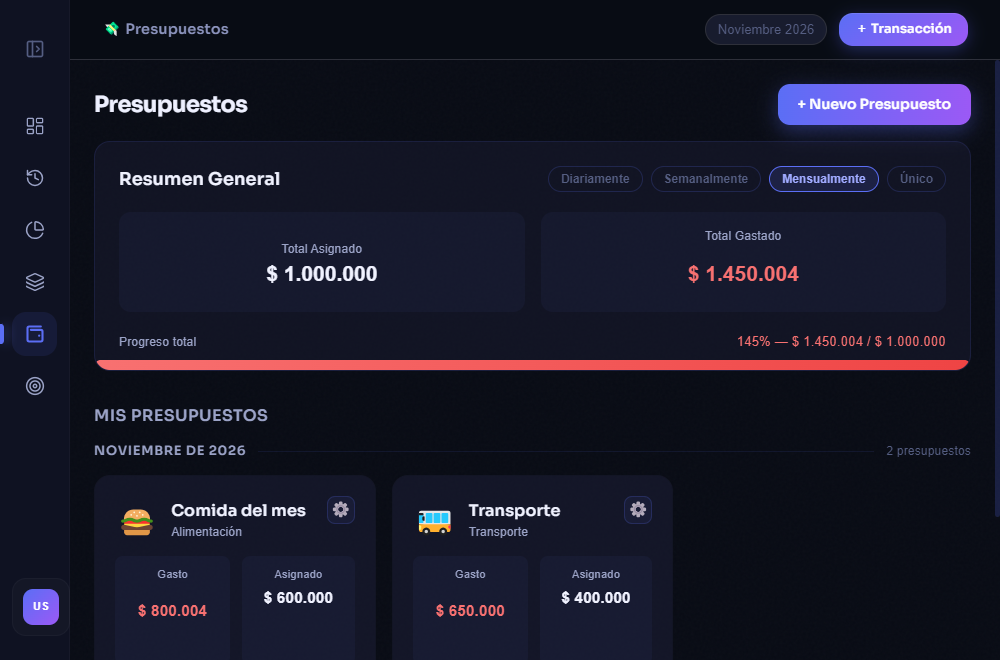
\includegraphics[width=0.8\linewidth]{../evidencias/cypress_e2e_presupuestos.png}
\figurenote{Fuente: elaboración propia con Cypress 13.17.0.}
\end{figure}

\begin{table}[H]
\caption{Evaluación de las pruebas de integración}
\label{tab:eval-integracion}
\footnotesize
\begin{tabularx}{\linewidth}{L{3.6cm} Y Y}
\toprule
Medida & Primera ejecución (25/10/2026) & Segunda ejecución (21/11/2026) \\
\midrule
Casos & 11 (PI-01 a PI-10 y E2E) & 18 (PI-01 a PI-17 y E2E) \\
Aprobados & 6 & 18 \\
Fallidos & 3 (PI-04, PI-09, PI-10) y 1 parcial (PI-05) & 0 \\
Pendientes & 1 (PI-08) & 0 (PI-05 en PostgreSQL queda pendiente) \\
Cypress & 8 pruebas: 7 aprobadas, 1 fallida (PI-04) & 8 pruebas: 8 aprobadas \\
Defectos & D-03, D-04, D-05, D-07 confirmados & D-11 y D-12 encontrados y corregidos \\
\bottomrule
\end{tabularx}
\tablenote{Fuente: elaboración propia.}
\end{table}

\subsection{Defectos encontrados, corrección y reprueba}

\begin{table}[H]
\caption{Defectos de integración: corrección y reprueba}
\label{tab:defecto-correccion}
\footnotesize
\begin{tabularx}{\linewidth}{L{1cm} L{3.2cm} Y L{3.2cm}}
\toprule
ID & Defecto & Corrección & Reprueba \\
\midrule
D-03 & \codigo{month} fuera de 1–12 daba 500 & Validadores de mes (1–12) y año (2000–2100) en \codigo{schemas.py} & PI-09 aprobada \\
D-04 & Porcentaje limitado a 100 & \codigo{budget_service.percentage_used} devuelve el valor real; el frontend solo limita el ancho de la barra & PI-04 aprobada \\
D-05 & FK \codigo{NOT NULL} con \codigo{SET NULL} & \codigo{ON DELETE RESTRICT} y 409 en \codigo{delete_category} & PI-05 aprobada (SQLite) \\
D-07 & Meta sin fecha final daba 500 & \codigo{create_goal} guarda la fecha por defecto (30 días) & PI-10 aprobada \\
D-11 & Borrar cuenta o categoría con datos daba 500 & \codigo{cascade="all, delete-orphan"} en las relaciones del ORM & PI-13 aprobada \\
D-12 & Editar una transacción aceptaba una categoría ajena & \codigo{update_transaction} usa \codigo{get_accessible_category} & PI-14 aprobada \\
\bottomrule
\end{tabularx}
\tablenote{El registro completo de defectos está en el Apéndice \ref{ap:defectos}. Fuente: elaboración propia.}
\end{table}

\paragraph{Conclusión.} La integración incremental permitió aislar cada defecto en su capa: D-03 y D-07 en la validación (N2), D-04 en los servicios (N3), D-05 y D-11 en la persistencia (N1) y D-12 en las rutas (N4). Tras las correcciones, los 18 casos pasan con pytest y Cypress. La migración de la clave foránea ya se aplicó en Supabase, así que la base de producción cumple la misma regla que verifica PI-05.
